\documentclass[review]{elsarticle}

\usepackage{lineno,hyperref}
\modulolinenumbers[5]
%\usepackage[margin=2cm]{geometry}
\usepackage[justification=centering]{caption}
\usepackage{subfig}
\usepackage{multirow}
\journal{Pattern Recognition}

%%%%%%%%%%%%%%%%%%%%%%%
%% Elsevier bibliography styles
%%%%%%%%%%%%%%%%%%%%%%%
%% To change the style, put a % in front of the second line of the current style and
%% remove the % from the second line of the style you would like to use.
%%%%%%%%%%%%%%%%%%%%%%%

%% Numbered
%\bibliographystyle{model1-num-names}

%% Numbered without titles
%\bibliographystyle{model1a-num-names}

%% Harvard
%\bibliographystyle{model2-names.bst}\biboptions{authoryear}

%% Vancouver numbered
%\usepackage{numcompress}\bibliographystyle{model3-num-names}

%% Vancouver name/year
%\usepackage{numcompress}\bibliographystyle{model4-names}\biboptions{authoryear}

%% APA style
%\bibliographystyle{model5-names}\biboptions{authoryear}

%% AMA style
%\usepackage{numcompress}\bibliographystyle{model6-num-names}

%% `Elsevier LaTeX' style
\bibliographystyle{elsarticle-num}
%%%%%%%%%%%%%%%%%%%%%%%

\begin{document}

\begin{frontmatter}

\title{Automatize landmarks detection with Deep Learning}
%\tnotetext[mytitlenote]{Fully documented templates are available in the elsarticle package on \href{http://www.ctan.org/tex-archive/macros/latex/contrib/elsarticle}{CTAN}.}

%% Group authors per affiliation:
%\author{Elsevier\fnref{myfootnote}}
%\address{Radarweg 29, Amsterdam}
%\fntext[myfootnote]{Since 1880.}

%% or include affiliations in footnotes:
\author[labri,itdlu]{Le Van Linh\corref{cor1}}
\ead{van-linh.le@labri.fr}
\author[labri]{Beurton-Aimar Marie\fnref{ba}}
\author[labri]{Zemmari Akka}
\author[igepp]{Parisey Nicolas\fnref{ba}}

\fntext[ba]{both authors contributed equally to this work.}
\cortext[cor1]{Corresponding author} 

\address[labri]{University of Bordeaux, 351, cours de la Libération, 33405 Talence, France}

%% %% or include affiliations in footnotes:
\address[igepp]{UMR 1349 IGEPP, BP 35327, 35653 Le Rheu, France}
%% \ead[url]{www.elsevier.com}
\address[itdlu]{Dalat University, Dalat, Lamdong, Vietnam}

\begin{abstract}
Landmark is one of the important concepts in Procrustes Analysis. Finding landmarks is not only used to measure the shape of the object, but also applied to determine the correspondence between the objects when applying the alignment methods. 
In biology, landmarks are widely used in the morphometric analysis. They are used to analyze the inter-organisms variations. The main objective is to classify and to determine the evolution of an organism's family. 
Currently, the landmarks are mostly determined manually by the biologist.
In this work, we applied Deep Learning, specify Convolutional Neural Network (CNN), to predict the landmarks on biological images.
Whereby, we proposed a CNN architecture which was built from the ``elementary blocks". Each block is made up of some popular layers of CNN.
The network then will be trained and tested on a dataset includes five parts of beetle (head, elytra, pronotum, left and right mandibles).
These works have also introduced another strategy to augment the dataset which can see a little bit small in our case.
In the experiments, we apply two strategies to evaluate the network and to improve the obtained results: training from scratch and applying a fine-tuning step.
The predicted landmarks from the network will be compared with the manual landmarks which provided by the biologists.
The obtained results are considered to be statistically good enough to replace the manual landmarks. The complete workflow is implemented and freely available on GitHub.
\end{abstract}

\begin{keyword}
Landmarks \sep deep learning \sep fine-tuning \sep CNN
\end{keyword}

\end{frontmatter}

\linenumbers

\section{Introduction}
\label{sIntroduction}

Anatomical landmarks are preferred to the points that represent a biological object. They have a biologically meaningful point in an organism and are widely used to ensure the correspondences within the same species. The anatomical landmarks are used in many biological studying, the biologist can estimate the shape from the collected landmarks, then they may evaluate the evolution of a group organism. Depending on which kind of analysis objects, the number of landmarks may different, as well as their positions can be defined along the shape or inside the object, i.e. Drosophila wings (Fig. \ref{imgflywing}) have $13$ landmarks and they are located on the veins of the wings, while the head of a beetle has $10$ landmarks and they stay inside the object (Fig. \ref{figbt3}).

Currently, the landmarks on anatomical images are set manually by the entomologist. One thing can note that the manual work is very time-consuming and difficult to reproduce when the users change the operations. In other scenes, some methods have been applied to estimate the landmarks automatically on anatomical images \cite{lowe2004distinctive, bay2006surf, palaniswamy2010automatic}. In these methods, a sequence of image processing techniques have been hired to finish the estimation, i.e. SIFT \cite{lowe2004distinctive}, SURF \cite{bay2006surf} are including 4 steps to give the estimated landmarks. It is worth noting that if a step in these procedure provides a bad result, it will affect the final result and it will become a bottleneck of the method. For example, segmentation is the most important step in image processing. In some cases, the object in the image is easy to extract and we can analyze the object with the help of well-known image analysis procedures. But in other cases, when the image is noisy, applying segmentation will not give any hope. In the previous study \cite{le2017maelab}, we have studied two anatomical parts of the beetle: left and right mandibles. These parts just contain the interested object and pretty easy to segment. So, sequence algorithms have been applied to estimate the landmarks and they have provided good results. However, the results are not the same when we applied the same method to other parts of beetle, i.e. pronotum. So, considering a method to predict the landmarks without helping of segmentation step is needed. 

In this work, we propose a CNN \cite{lecun2010convolutional} which consists of several ``elementary block". Each block is built from the popular layers in CNN, i.e. convolutional layer, max pooling layer, and dropout layer. After designing, the proposed model will be trained on the dataset includes the images which are taken from $293$ beetles. For each beetle, the biologists have taken images of five parts: \textit{left and right mandibles, head, elytra, and pronotum} (Fig. \ref{figbeetle}). All the images are presented in the RGB color model with two dimensions. Along with each image, a set of landmarks has been marked by experts which can be used as ground truth to evaluate the predicted landmarks. During the experiments, the proposed network has been trained on the dataset by applying two strategies. In the first strategy, the network is trained from scratch on each dataset of each part; while in the second strategy, the training process has been modified to include a fine-tuning \cite{yosinski2014transferable} stage. The proposed network will be trained on the combining data of some parts, i.e. pronotum, elytra, and head, to obtain the pre-trained model. Then, the pre-trained model will be fine-tuned on each dataset. Besides, the value of Root Mean Square Error (RMSE) is used to compute the loss during two experiment processes. For more information about the model, you can see at our repository on GitHub: \texttt{https://github.com/linhlevandlu/CNN\_Beetles\_Landmarks}.

\begin{figure}[htbp]
    \centering
    \subfloat[Left mandible]{\label{figbt1}		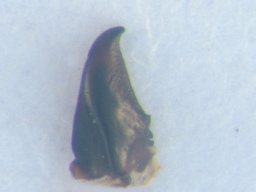
\includegraphics[width=0.45\textwidth]{images/mg019}}~~
\subfloat[Right mandible]{\label{figbt2}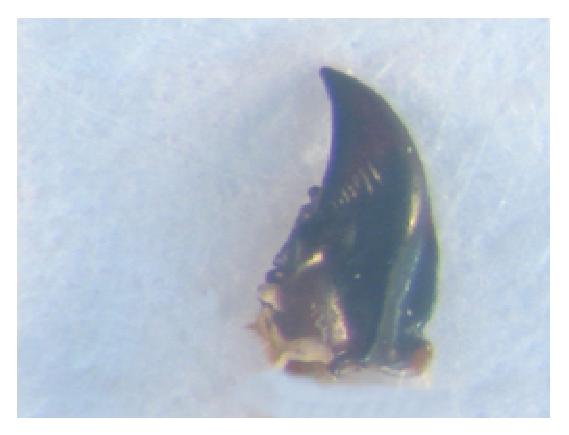
\includegraphics[width=0.45\textwidth]{images/md19}}\\
	\subfloat[Head]{\label{figbt3}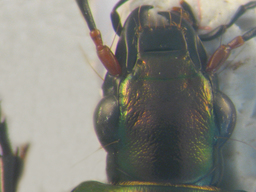
\includegraphics[width=0.45\textwidth]{images/tete081}}~~
\subfloat[Pronotum]{\label{figbt4}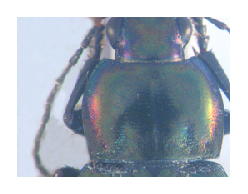
\includegraphics[width=0.45\textwidth]{images/prono60}}\\
	\subfloat[Elytra]{\label{figbt5}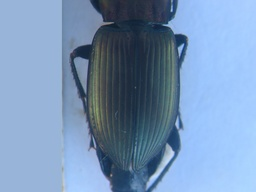
\includegraphics[width=0.45\textwidth]{images/elytre107}}    
    \caption{The anatomical images of beetle are taken into account.}
    \label{figbeetle}
\end{figure}

The rest of this paper is organized as followed: Section \ref{related_works} discusses the related works of automatic estimation landmarks on 2D images. The, the dataset and the method which use to augment the dataset will be presented in Section \ref{Sdataaug}. Section \ref{Sneuralnetwork} shows the procedure of designing the network model. The first experiment of the network on each dataset is presented in Section \ref{sexperiments}. Section \ref{sfineTuning} presents a modification of training process and its experiment on datasets.
Finally, the conclusion is given in Section \ref{sconclusion}.

\section{Related works}
\label{related_works}
In geometric morphometry, landmarks (or points of interest) are important features to describe the shape. Depending on the complicacy of the objects in the image, setting automatic landmarks can rely on different methods. When the object can be segmented, the image processing techniques may applied to predict the landmarks. Lowe et al. \cite{lowe2004distinctive} have proposed SIFT method to identify the keypoints on 2D images by extracting the distinctive features from the images. It is composed by four steps: (1) scale space extrema detection: a difference of Gaussian (DoG) function is applied to identify the interested points at all scales; (2) keypoint localization: the keypoint candidates are localized and refined by deleting the points which have the low contrast or not localized along the edge; (3) orientation assigment: for each keypoint candidates, the orientation and gradient magnitude are computed by considering their 4-neighborhoods; (4) keypoint descriptor are computed for each keypoint from its orientation and gradient magnitude. From the descriptors of the keypoints, they can be used to find the corresponding points between two images. SURF is another method which has been proposed by Herbert Bay et al. \cite{bay2006surf}. The SURF algorithm is the same principles with SIFT but details in each step are different. This algorithm mainly has three steps: (1) keypoints detection, (2) local neighborhood description and (3) matching. Different with SIFT, SURF uses a blob detector base on the Hessian matrix to find the keypoints. The Hessian matrix is used as a measure of local change around the point and chooses the points where this determinant is maximal. Then, the descriptors are computed around the key points by describing the intensity distribution of keypoint's neighborhoods. The matching points from different images are obtained by comparing the descriptors of the key points. Palaniswamy et al. \cite{palaniswamy2010automatic} have proposed a method to automatically detect the landmarks on 2D images of Drosophila wings (Fig. \ref{imgflywing}). The method is mainly based on probabilistic Hough Transform. It includes four steps: (1) features detection of the fly wing structure (segmentation); (2) using pairwise geometric histogram (PGH) to record the compact invariant shape descriptor; (3) estimating the global pose of wing using the probabilistic Hough transform; (4) and finally a template matching is applied to refine the correctly of individual features.

\begin{figure}
	\centering
	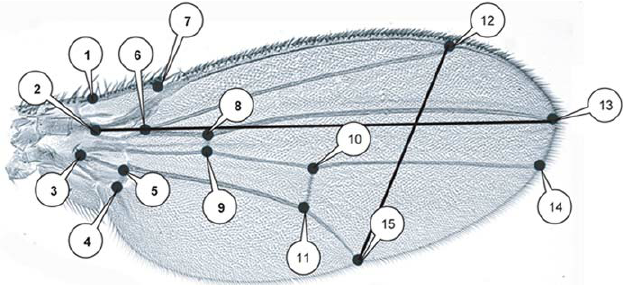
\includegraphics[scale=.4]{images/wing_landmarks}	
	\caption{A Drosophila wing and its landmarks}
	\label{imgflywing}
\end{figure}

In recent years, deep learning \cite{lecun2015deep} is known as a solution for the tasks in computer vision, especially for image analysis. Deep learning has been introduced in the middle of the previous century for artificial intelligence application but it has encountered several problems to take real-world cases. Luckily, the improvement of computing capacities, both in memory size and computing time with GPU programming, has opened a new perspective for deep learning. Many deep learning architectures have been proposed to sovle the problems of classification \cite{krizhevsky2012imagenet, ciregan2012multi}, image recognition \cite{szegedy2015going, farabet2013learning, li2015convolutional}, speech recognition \cite{mikolov2011strategies, hinton2012deep}, language translation \cite{jean2014using, sutskever2014sequence}, \ldots. Using deep learning, specifically CNN, to predict the landmarks on 2D images has achieved better results even if the images that can not segment. Yi Sun et al. \cite{sun2013deep} have proposed a cascaded CNNs to predict the facial points on the human face. Their model includes the networks which have separated into three levels of the cascade. The networks recognize the human face from the global to the local view to increasing the accuracy of predicted key points. Zhanpeng Zhang et al. \cite{zhang2014facial} proposed a \textit{Tasks-Constrained Deep Convolutional Network} to optimize facial landmarks detection. Their model detected the facial landmarks with a set of related tasks such as head pose estimation, gender classification, age estimation, or facial attribute inference. Cintas et al. \cite{cintas2016automatic} has introduced a network to predict the landmarks on human ears (Fig. \ref{imgears}). After training, the network has the ability to detect $45$ landmarks on human ears. 

\begin{figure}[!h]
	\centering
	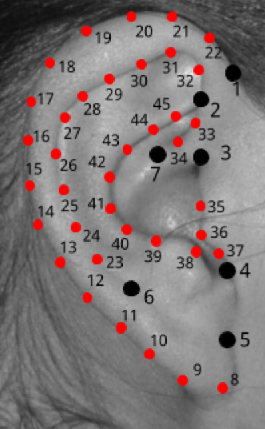
\includegraphics[scale=.4]{images/ear_landmarks}	\
	\caption{Landmarks on human ear in study of Cintas et al. \cite{cintas2016automatic}}
	\label{imgears}
\end{figure}


As an association with the biologist, we study to develop an automatic method for predicting the landmarks on beetle's anatomical (Fig. \ref{figbeetle}). As we can see in this section, the methods for landmarking can be divided into two groups by considering the techniques that they have used. Most of the methods in the first group choose the image processing techniques while other methods are used deep learning. In a previous work \cite{le2017maelab}, we have applied a series of algorithms to detect the landmarks automatically on beetles mandibles which are considered as the easied objects to segment (with an quality enough good for our need). In that work, the landmarks have been detected by registering two segmentations of images and then, using SIFT descriptor to refine the location of predicted landmarks. After the experiment, we have obtained good enough results on mandibles. Unfortunately, we have observed that the method did not provide good results when the segmentation is not precise, i.e. on pronotum or elytra images. This is explained why we have turned the automatically landmarking into another stage without any segmentation step. Using CNN for landmarking seems that a good choice for un-segmentable images.

In deep learning, the dataset is also an important component along with the network. Training a network on a large dataset will improve the learnable of the network because dataset has provided more different cases to learn. However, we are not always have enough data for training in practice.. Instead of, the user applies some techniques to augment the dataset. Our case is not an exception, we work on a small dataset with 293 images of each part. This number is really modest with deep learning. So, a method has been through to augment the dataset. This procedure will be presenting in the next section.

\section{Data augmentation}
\label{Sdataaug}
A characteristic of machine learning and deep learning is using a volume dataset to train the model. The question is how do we can apply deep learning if we have a limitation dataset? One way to solve this problem is to create the fake data from real data and to add it to the training set. Dataset augmentation has been a particularly effective technique for a specific problem. For example, in images classification problem, the operations like translating,  rotating or scaling the images have also effective. The fake images may be generated by translating (rotating or scaling) in each direction. Besides, injecting noise in the input can also see as a form of data augmentation.

Our dataset includes $293$ images of beetles (for each anatomical part). All the images are taken with the same camera in the same condition with a resolution of $(3264 \times 2448)$. Each image has a set of manual landmarks provided by biologists, i.e, each pronotum has $8$ landmarks, each head has $10$ landmarks. Applying CNNs to train each part with a small number of images to reach good results is impossible. So, we need to augment the dataset before training the networks. Firstly, we have found that the original solution of the images $(3264 \times 2448)$ are heavy for the neural network. For performance considerations, in most of CNNs \cite{cintas2016automatic, lecun2010convolutional, sun2013deep}, the size of the input is limited to $(256 \times 256)$ pixels, so we have decided to down-sampling the images to a new resolution $(256 \times 192)$ (to respect the ratio between $x$ and $y$). Of course, the coordinates of manual landmarks have been also scaled to fit with the new resolution of the images. In usual way, the transformations have been used to augment the dataset (i.e rotation, translation,\ldots) but the analysis of image by CNN is most often translation and rotation invariant. Therefore, two other procedures have been imaged to increase the number of images in the dataset $(256 \times 192)$.

The first procedure is to change the value of a color channel in the original image to generate a new image. According to that, a constant is added to one of the RGB channels each time it is used for training. Each constant is sampled in a uniform distribution $\in [1, N]$ to obtain a new value caped at $255$. For example, Fig. \ref{figaug1} shows an example when we added a constant $c = 10$ to each channel of an original image. Following this way, we can generate three version from an image.

\begin{figure}[h]
	\centering
	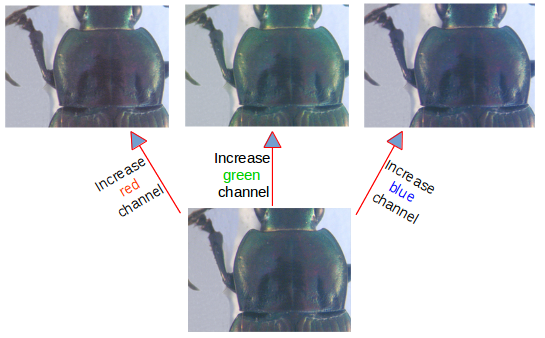
\includegraphics[scale=0.35]{images/inc_channels}
	\caption{A constant $c = 10$ has been added to each channel of an original image}
	\label{figaug1}
\end{figure}

In the second procedure, we have applied the opposite procedure to the first one. Instead of adding the value, we separate the channels of RGB into three gray-scale images as the network works on single channel images (Fig. \ref{figaug2}). At the end of the processes, we are able generate six versions from an original image. In total, we have $293 \times 7 = 2051$ images for each anatomical part of beetle (an original image and six generated images). However, we have not used all images for training and validation. So, we have chosen $260$ original images and their generations ($1820$ images) of each dataset for training and validation processes, the remaining images ($33$ original images) are used for test process.

\begin{figure}[h]
	\centering
	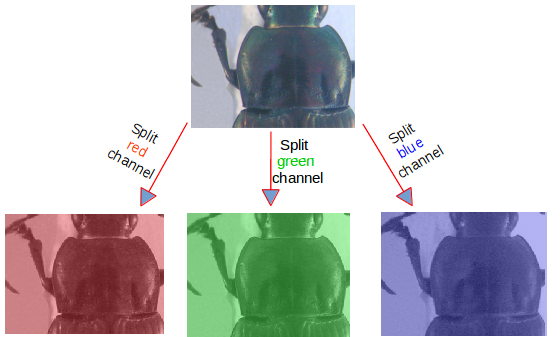
\includegraphics[scale=0.35]{images/sp_channels}
	\caption{Three channels (red, green, blue) are separated from original image}
	\label{figaug2}
\end{figure}

In practical, to obtain a fast convergence during the computing, it is useful to normalize the brightness of the images to $[0,1]$ instead of $[0, 255]$ and the coordinates of the landmarks have been also normalized \cite{lecun2012efficient}.

\section{Network architectures designing}
\label{Sneuralnetwork}
In the process, we have tried three network models before deciding the final architecture for detecting the landmarks on beetle images. Like other CNN models, we have employed the classical layers to construct the models, i.e., convolutional layers, maximum pooling layers, dropout layers and full-connected layers.

The first architecture is very classical one, it receives an image with the size of $(1 \times 192 \times 256)$ as the input. Then, the network consists on three repeated strucutre of a convolutional layers followed by a maximum pooling layers. Most CNNs, the hyperparameters of convolutional layers have been set to increase the depth of the images from the first layer to the last layer. That is reflected in the setting of the number of filters at each convolutional layer. So, the depths of convolutional layers increase from $32, 64, $ and $128$ with different size of the kernels: $(3 \times 3)$, $(2 \times 2)$ and $(2 \times 2)$, respectively. Inserting pooling layers after a convolutional layers is a common periodcally. The pooling layer effects to progressively reduce the spatial size of the representation to reduce the number of parameters, computation in the network, and it also controls over-fitting. The operations of pooling layers independent on every depth slice of the input. The most common form is a pooling layer with filters of size $(2 \times 2)$ and a stride of $2$. It downsamples every depth by $2$ along width and height of the input. Thefore, all the kernels of maximum pooling layers have the same size of $(2 \times 2)$ with a stride of $2$ as usual. At the end of the model, three full-connected layers have been added to extract the global relationship between the features and to procedure the outputs. The first of two full-connected layers are set to non-linearity to make sure these nodes interact well and take into account all possible dependencies at the feature level. The outputs of the full-connected layers are $500, 500$ and $16$. The output of the last full-connected layer corresponds to the coordinates ($x$ and $y$) of $8$ landmarks which we would like to predict. Fig. \ref{fignet1} shows details of the first model: The orange rectangles represent for convolutional layers while the yellow rectangles represent for maximum pooling layers and three full-connected layers with their parameters are presented at the end of the model.

\begin{figure}[!h]
	\centering
	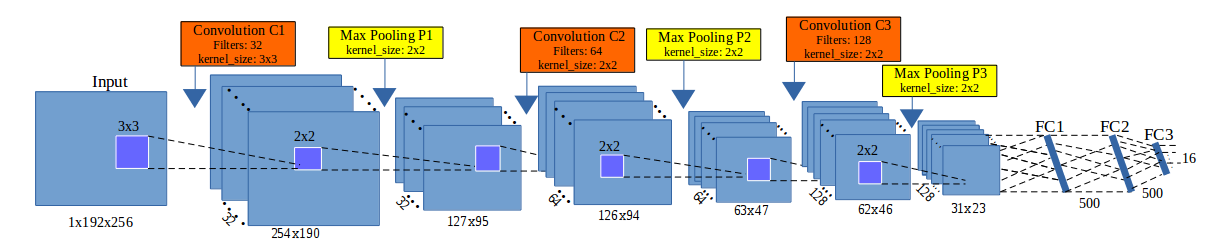
\includegraphics[scale=0.3]{images/net1}
	\caption{The architecture of the first model}
	\label{fignet1}
\end{figure}

The second architecture is modified from the first model. The layers are kept the same as the first one but the outputs of the first of two full-connected layers are changed from $500$ (in the first model) to $1000$ (Fig. \ref{fignet2}). Increasing the value at full-connected layers is hoping to obtain more features from convolutional layer and to prevent the over-fitting. 

\begin{figure}[h]
	\centering
	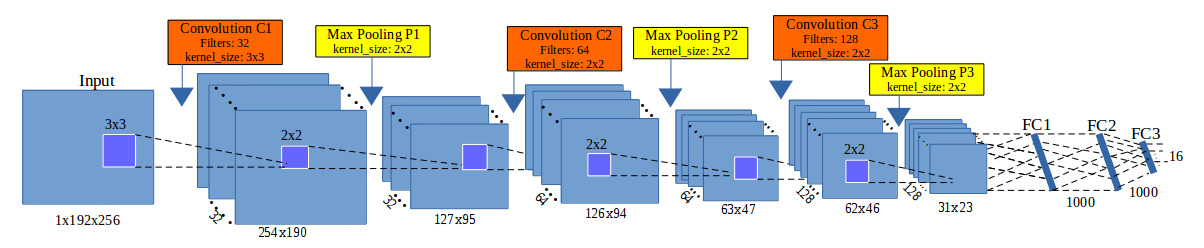
\includegraphics[scale=0.3]{images/net2}
	\caption{The architecture of the second model}
	\label{fignet2}
\end{figure}

To build the third architecture, we have used the definition of \textit{elementary block}. An {elementary block} is defined as a sequence of convolution ($C_{i}$), maximum pooling ($P_i$) and dropout ($D_i$) layers (Fig. \ref{figelementary}). This significantly reduces overfitting and gives major improvements over other regularization methods \cite{srivastava2014dropout}. The idea of dropout is to include some variations between different runs. During training phase, dropout samples are done from an exponential number of different ``thinned" network. At test phase, it is easy to approximate the effect of averaging the prediction of all thinned networks by simply using a single unthinned network with smaller weights. So, we have modified the architecture by combining some \textit{elementary blocks}. 

\begin{figure}[h]
	\centering
	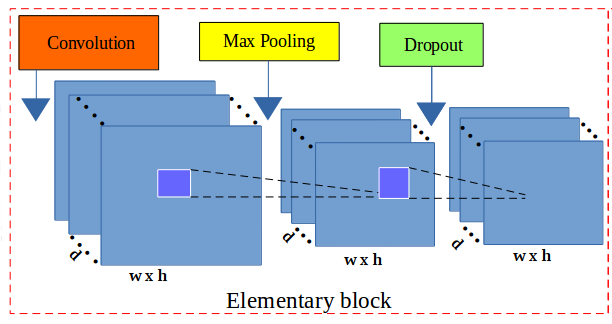
\includegraphics[scale=0.3]{images/elementary_block}
	\caption{The layers in an elementary block}
	\label{figelementary}
\end{figure}

Fig. \ref{fignet3} illustrates the layers in the third architecture. For our purpose, we have assembled \textbf{3 elementary blocks}. The parameters for each layer in each elementary block are as below, the list of values follows the order of elementary blocks ($i = [1..3]$):
\begin{itemize}
	\item CONV layers:
	\begin{itemize}
		\item Number of filters: $32, 64, $ and $128$
		\item Kernel filter sizes: $(3 \times 3), (2 \times 2), $ and $(2 \times 2)$
		\item Stride values: $1, 1, $ and $1$
		\item No padding is used for CONV layers 
	\end{itemize}
	\item POOL layers:
		\begin{itemize}
			\item Kernel filter sizes: $(2 \times 2), (2 \times 2), $ and $(2 \times 2)$
			\item Stride values: $2, 2, $ and $2$
			\item No padding is used for POOL layers
		\end{itemize}
	\item DROP layers:
		\begin{itemize}
			\item Probabilites: $0.1, 0.2, $ and $0.3$
		\end{itemize}
\end{itemize}

Three full-connected layers (FC) are kept the same as the second architecture: FC1 and FC2 have $1000$ outputs, the last full-connected layer (FC3) has $16$ outputs. As usual, a dropout layer is inserted between FC1 and FC2 with a probability equal to $0.5$.
\begin{figure}[h]
	\centering
	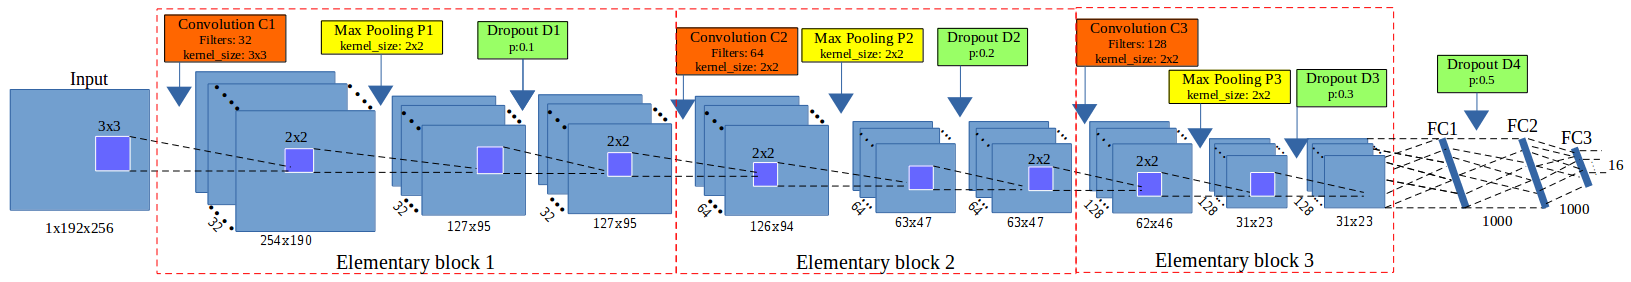
\includegraphics[scale=0.2]{images/arch_model}
	\caption{The architecture of the third model}
	\label{fignet3}
\end{figure}

The core of neural network is training over iteration. There are many ways to optimize the learning algorithm, but gradient descent \cite{lecun2012efficient} is currently a good choice to establish the way of optimizing the loss in neural network. The core idea is following the gradient until we statify with the results will remain the same. So, we have chosen gradient descent in the backward phase to update the values of learnable parameters and to increase the accuracy of the network. The networks are designed with a small sharing learning rate and a momentum. The learning rate is initialized at $0.03$ and stopped at $0.00001$, while the momentum is updated from $0.9$ to $0.9999$. Their values are updated over training time to fit with the number of epochs \footnote{An epoch is a single pass through the full training set}. The implementation of the architectures have been done on Lasagne framework \cite{lasagne} by Python. 

\section{Experiments and results}
\label{sexperiments}
Before widely applying to all anatomical parts, we have firstly tried with pronotum part to evaluate the performance. The networks have been trained in $5, 000$ epochs on Ubuntu machine by using NVIDIA TITAN X cards. The set of images that used for training and validation are merged together. During the training, the images are chosen randomly from the dataset with a ratio of $60\%$ for training and $40\%$ for validation. The training step takes into account a pair of information (\textit{images, manual landmarks coordinates})  as training data. In the context of deep learning, landmark prediction can be seen as a regression problem. So, we have used Root Mean Square Error (RMSE) to compute the loss of implemented architectures. At the test phase, images without landmarks are given to the trained network to produce output coordinates of the predicted landmarks. The results then evaluated by comparing with the manual landmarks coordinates provided by biologists which have been seen as ground truth. 

Fig. \ref{figloss1} shows the training errors and the validation errors during traning phase of the first architecture. The blue curve presents the RMSE errors of training process while green curve is the validation errors. Clearly, over-fitting has appeared in the first model. The training losses are able to decrease but the validation losses are stable. In the second model (section \ref{Sneuralnetwork}), we have modified the parameters of full-connected layers to prevent the over-fitting but it seems that this solution is still not suitable.

\begin{figure}[!h]
	\centering
	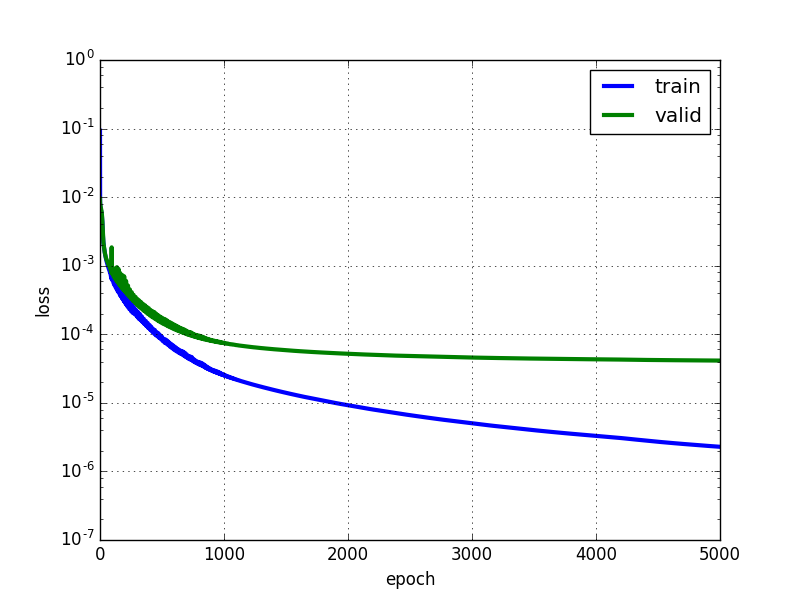
\includegraphics[scale=0.4]{images/cnnmodel3_5000_pronotum_v13_without_dropout_normalized_data_loss}
	\caption{The training and validation losses of the first model}
	\label{figloss1}
\end{figure}

Then, we have continued to train the third model on the same dataset of pronotum images. Fig. \ref{figloss2} illustrates the losses during the training of the third model. Like the previous figure (Fig. \ref{figloss1}), the blue line is training losses, the green line is validation losses. In the opposite with two previous models, the losses are different (far) from the beginning but after several epochs, the values become more proximate and the over-fitting problem has been solved. This proves that adding dropout layers to build the elementary blocks have been effects to prevent over-fitting and contributory improve the accuracy of the model. \textit{So, we have decided to keep the architecture of the third model for our landmarking problem.}

\begin{figure}[!h]
	\centering
	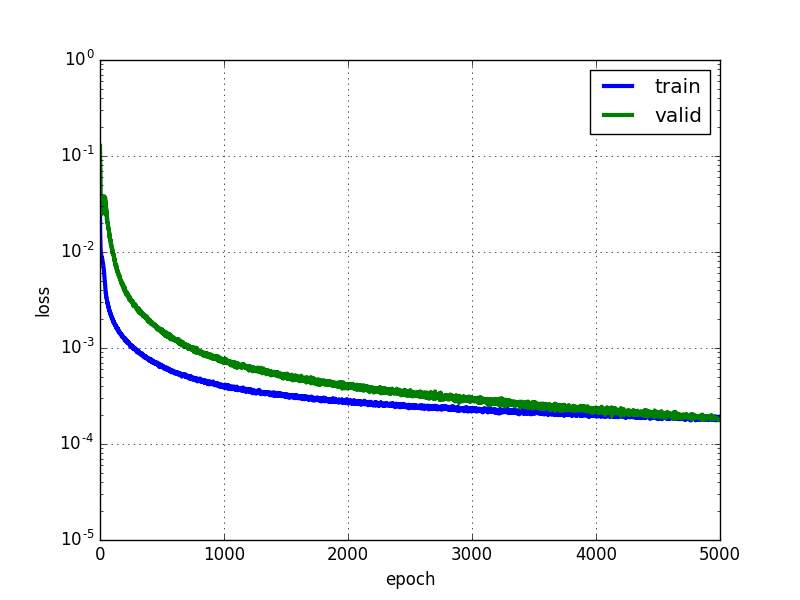
\includegraphics[scale=0.4]{images/loss_v16}
	\caption{The training and validation losses of the third model}
	\label{figloss2}
\end{figure}

In order to have the predicted landmarks for all pronotum images (instead of only $33$ images), we have applied \textit{cross-validation} to choose the test images, called \textit{round}. For each time, we have chosen a different fold of $33$ images as testing images, the remaining images are used as training and validation images ($293/33 \approx 9$ rounds). Following that, the network will be trained with different datasets, then the trained model will be used to predicted the lanmarks on the images in the corresponding test set. Table. \ref{tbltrainingloss} resumes the losses of $9$ rounds when we trained the third model on pronotum images. From the Table. \ref{tbltrainingloss}, the losses among the rounds are stable (i.e $\approx 0.00020$ for traning loss and $\approx 0.00024$ for validation loss), they have a different but not so large. According that, the RMSE values are looking pretty good ($\approx 1.7 - 2.1$ pixels).

\begin{table}[h!]
	\centering
	\begin{tabular}{l l l}
	Round & Training loss & Validation loss \\ \hline
	1 & 0.00018 & 0.00019  \\ \hline
	2 & 0.00019 & 0.00021 \\ \hline
	3 & 0.00019 & 0.00026 \\ \hline
	4 & 0.00021 & 0.00029 \\ \hline
	5 & 0.00021 & 0.00029 \\ \hline
	6 & 0.00019 & 0.00018 \\ \hline
	7 & 0.00018 & 0.00018 \\ \hline
	8 & 0.00018 & 0.00021 \\ \hline
	9 & 0.00020 & 0.00027 \\ \hline
	\end{tabular}
	\caption{\small{The losses during training the third model on pronotum images}}
	\label{tbltrainingloss}
\end{table}

To evaluate the coordinates of predicted landmarks, the correlation metrics have been computed the correlation between the manual landmarks and their corresponding predicted one. Table. \ref{tblcorrelation} shows the correlation scores of $3$ metrics (using \textit{scikit-learn} \cite{pedregosa2011scikit}), i.e, coefficient of determination ($r^2$), explained variance (EV), and Pearson correlation. All of three metrics have the same possibility. The best score is $1.0$ if the correlation data is good, lower values are worse. It means that our predicted coordinates are very close with the ground truth. However, the measure is not enough good to provide a useful result to biologists. Moreover standing on the side of image processing, we are looking forward to  seeing the predicted coordinates than the statistical results.

\begin{table}[htbp]
	\centering
	\begin{tabular}{|c|p{2cm}|p{2cm}|p{2cm}|}
		Metric & $\mathbf{r^{2}}$ & \textbf{EV} & \textbf{Pearson} \\ \hline
		Score & $\textbf{0.9952}$ & $\textbf{0.9951}$ & $\textbf{0.9974}$ 
	\end{tabular}
	\caption{Correlation scores between manual landmarks and predicted landmarks}
	\label{tblcorrelation}
\end{table}

The main goal of computing is to predict the coordinates of landmarks, so the distances (in pixels) between the coordinates of manual landmarks and corresponding predicted landmarks have been taken into account on all images. Then, the average of distances are computed by landmarks. Table. \ref{tblavgthorax} shows the average distances by landmarks on all images of pronotum dataset. With images of resolution $256 \times 192$, we can
consider that an error of $1\%$ corresponds to $2$ pixels that could
be an acceptable error. Unhappily, our results exhibit average
distance of $4$ pixels in the best case, landmark $1$ and more than
$5$ pixels, landmark $6$. Other error distances are more than $2\%$
pixels.

\begin{table}[htbp]
	\centering	
	\begin{tabular}{|c|c|}
		\hline
		\textbf{Landmark} & \textbf{Distance} (in pixels) \\ \hline
		1 & 4.002  \\ \hline
		2 & 4.4831 \\ \hline
		3 & 4.2959 \\ \hline
		4 & 4.3865 \\ \hline
		5 & 4.2925 \\ \hline
		6 & 5.3631 \\ \hline
		7 & 4.636 \\ \hline
		8 & 4.9363 \\ \hline
	\end{tabular}
	\caption{The average distances on all images per landmark on pronotum images.}
	\label{tblavgthorax}
\end{table}

Fig. \ref{figchartlm1} shows the distribution of the distances on the first landmark of all images. The accuracy based on the distance in each image can be
separated into three spaces: the images have the distance less
than average value ($4$ pixels): $56.66\%$; the images have the
distance from average value to $10$ pixels ($5\%$ acceptable errors): $40.27\%$; and the images have the distance
greater than $10$ pixels: $3.07\%$.

\begin{figure}[htbp]
	\centerline{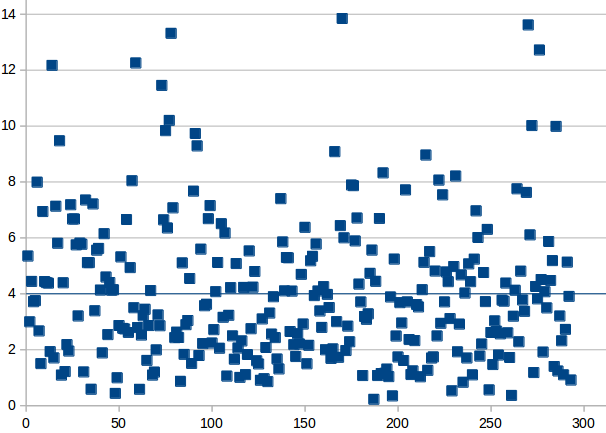
\includegraphics[scale=0.3]{images/statistic_pronotum_from_scratch_lm1}}
	\caption{The distribution of the distances on the first landmark. The blue line is the average value of all distances.}
	\label{figchartlm1}
\end{figure}

To illustrate this purpose, Fig. \ref{figrsexample} shows the predicted landmarks on two test images. One can note that even some predicted landmarks (Fig. \ref{figsub1}) are closed to the manual ones, in some case (Fig. \ref{figsub2}) the predicted ones are far from the expect results. This result explains why the average distance by landmarks are enough good while some predicted landmarks are so far from the manual one. So, the next step has been dedicated to the improvement of these results.

\begin{figure}[htbp]
    \centering
    \subfloat[Image with well-predicted landmarks]{\label{figsub1}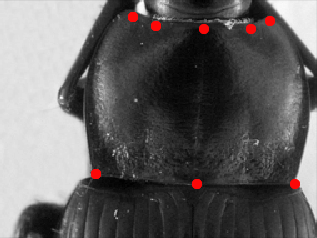
\includegraphics[width=0.35\textwidth]{images/fn_accuracy}}~~
\subfloat[Image with inaccuracy landmarks]{\label{figsub2}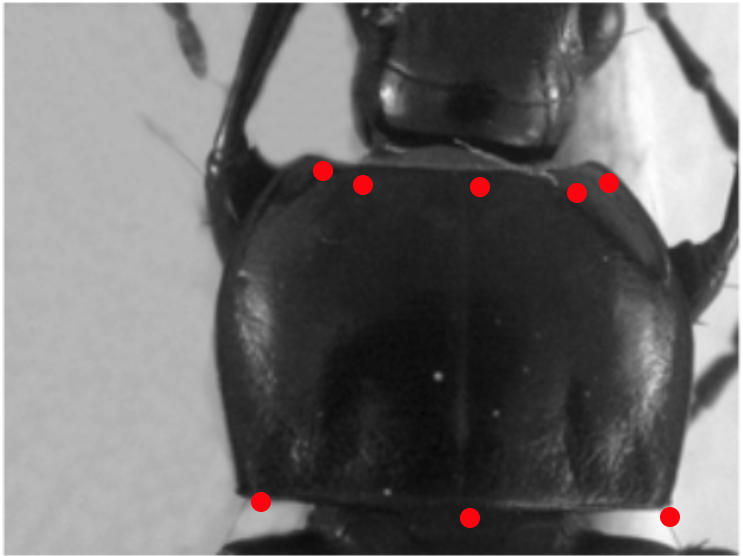
\includegraphics[width=0.35\textwidth]{images/plandmark2}}\\    
    \caption{The predicted landmarks, in red,  on the images in test set.}
    \label{figrsexample}
\end{figure}

From the success of the third architecture on pronotum dataset, we apply the same procedures (data augmentation, training,\ldots) on other parts of beetle: \textit{left and right mandibles, elytra and head}. However, we have modified the number of output of the last full-connected layer to adapt with each dataset before training. According, the values at the last full-connected layer are set to $32$, $36$, $22$ and $20$ outputs corresponds to $16$, $18$, $11$ and $10$ landmarks on left mandible, right mandible, elytra and head, respectively. Of course, we have also applied \textit{cross-validation} to select testing data to get all predicted landmarks for all images in each dataset. Then, the quality of predicted landmarks are evaluated by comparing with the corresponding manual landmarks (distance computation). Table. \ref{tblavg4parts} shows the average distances on each landmark of elytra, head, left and right mandibles anatomical, respectively. Comparing with the average distances on the pronotum part, it seems that the proposed architecture provides more accurate predictions on the elytra dataset, but the results are opposite on other datasets.

\begin{table}[htbp]
	\centering	
	\begin{tabular}{|c|c|c|c|c|}
		\hline
		\multirow{2}{*}{\textbf{Landmark}} & \multicolumn{4}{|c|}{\textbf{Distance (in pixels)}} \\ \cline{2-5}
		 & Right mandible & Left mandible & Elytra & Head  \\ \hline
		1 & 9.4981 & 9.1267 & 3.8669 & 5.528  \\ \hline
2 & 7.1657 & 6.7198 & 3.973 & 5.1609  \\ \hline
3 & 7.242 & 6.8704 & 3.9166 & 5.3827 \\ \hline
4 & 7.0436 & 6.7719 & 3.8673 & 5.0345 \\ \hline
5 & 7.1599 & 7.125 & 4.0151 & 4.8393 \\ \hline
6 & 7.5699 & 6.9441 & 4.8426 & 4.4516 \\ \hline
7 & 7.4251 & 7.3158 & 5.2125 & 4.7937 \\ \hline
8 & 7.6636 & 7.4142 & 5.4685 & 4.5322 \\ \hline
9 & 7.7906 & 7.5846 & 5.2692 & 5.1412 \\ \hline
10 & 8.0197 & 7.6349 & 4.0709 & 5.0564 \\ \hline
11 & 8.314 & 7.6873 & 3.9896 & - \\ \hline
12 & 8.1564 & 8.4248 & - & - \\ \hline
13 & 8.8879 & 7.9983 & - & - \\ \hline
14 & 9.1842 & 7.4919 & - & - \\ \hline
15 & 8.7875 & 7.7903 & - & - \\ \hline
16 & 8.3141 & 8.5198 & - & - \\ \hline
17 & 8.2866 & - & - & - \\ \hline
18 & 8.8928 & - & - & - \\ \hline
	\end{tabular}
	\caption{The average distances on all images per landmark on left mandible, right mandible, elytra and head images.}
	\label{tblavg4parts}
\end{table}

\section{Resulting improvement by fine-tuning}
\label{sfineTuning}
The proposed network (third architecture) presented in Section \ref{Sneuralnetwork} have been trained from scratch on five datasets of beetles (left mandible, right mandible, pronotum, elytra, and head). At the first step, the network was able to predict the landmarks on the images. But as we have discussed, even if the strength of the correlation seems to validate the results, when we display the predicted landmarks on the images, the quality of the predicted coordinates are also not enough precise, and the average error are also still high (of course, we have the distances are higher than the average distances).

In order to reach more acceptable results for biologists, we have broadened model with another step of deep learning: \textbf{transfer learning}. That is a method enables to re-uses the model developed for a specific task/dataset to lead another task (called \textit{target task}) with another dataset. This process allows rapid process and improves the performance of the model on the target task \cite{torrey2009transfer}. The most popular example has been given with the project ImageNet of Google \cite{imagenet_cvpr09} which has labeled several millions of images. The obtained parameter values which can be used in another context to classify another dataset, eventually very different dataset \cite{margeta_mri}. The name of this procedure to re-use parameters to pretrain a model is currently called \textbf{fine-tuning}.

Fine-tuning does not only replace and retrain the model on
the new dataset but also fine-tunes the weights of a trained
model by continuing the backpropagation. Unfortunately,
some rapid tests have shown that re-using ImageNet features
has not been relevant for our application. We have designed a
way to reproduce the method with our own data. It is worth
noting that of course the size of data to pre-train has drastically decreased. For our pre-training step, the network has been
trained on the whole dataset including the images of three parts
of beetle \textit{i.e pronotum, elytra and head}. Then, the trained model
has been used to fine-tune and test on each dataset.
\subsection{Data preparation and training}
The images training dataset is combined from the images of three sets: \textit{pronotum, elytra, and head} (after augmentation). When applying the training from the scratch, we have used cross-validation to select the data ($9$ folds). It means that for each dataset, we have some different training data and corresponding testing data. So, the images that use to train the model are just select from one of the folds in each dataset. Specifically, we have taken $1, 820$ images of each part. In total, it includes $5, 460$ images $(260 \times 7 \times 3)$. 

\begin{figure}[htbp]
	\centerline{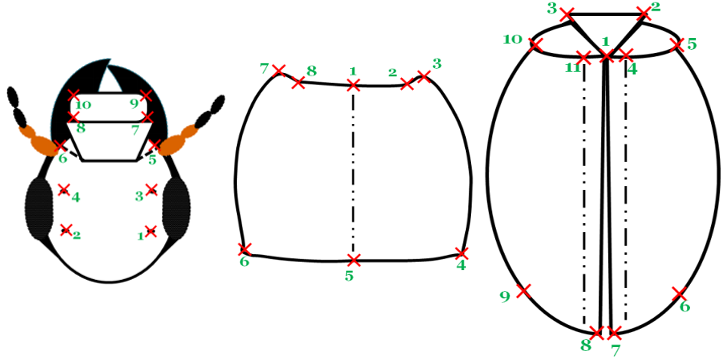
\includegraphics[scale=0.5]{images/merge}}
	\caption{A presentation of head, pronotum and elytra part with
corresponding manual landmarks}
	\label{figmerge}
\end{figure}

However, another problem has been appeared when we combined the images from different dataset. That is the different number of landmarks on each part: \textit{$8$ landmarks on pronotum part, $10$ landmarks on head part, and $11$ landmarks on elytra part}. Fig. \ref{figmerge} shows the possition of the landmarks on each part. Because of the meaning of landmarks on each anatomical part for biologists, we cannot insert the landmarks arbitrary. So,  we have decided to keep the landmarks on pronotum as reference and to remove the landmarks on elytra and head parts instead of adding. We kept $8$ (landmarks) as a reference number, then we have removed the supernumerary when it is unnecessary. Specifically, we have removed three landmarks on the elytra part ($1^{st}, 6^{th}, 9^{th}$), and two landmarks on the head part ($5^{th}, 6^{th}$). 

During training the proposed architecture on the combined dataset, the parameters of the network (learning rate, momentum, \ldots) are kept the same as training from scratch but the number of epochs are increased to $10, 000$ instead of $5, 000$ to achieve better learning on the parameters (weights). Additional, we have shuffled the training set. Because the neural network learns the faster from the most unexpected sample. It is advisable to choose a sample at each iteration that is the most unfamiliar to the system. Shuffling the examples will be helped the model works with different anatomical parts rather than the same anatomical samples in each training time.

\subsection{Fine-tuning on each dataset}
The combined dataset then used to train the third architecture with $16$ outputs ($8$ landmarks). Then, the trained model is used to fine-tuning on each dataset. To compare the result with the previous one, we have also fine-tuned the trained model with different dataset by applying cross-validation. Firstly, we consider on the losses during fine-tuning. \textit{For example}, Table. \ref{tblftpronotum}, \ref{tblftbody}, \ref{tblfthead} show the losses during fine-tuning on pronotum, elytra, and head dataset, respectively. Comparing with the losses when we trained the model from scratch, \textit{i.e.} on pronotum, the validation losses of all round in this scenario have been significantly decreased (around $40\%$).

On each part, the landmarks are predicted on the test images. Then, the average error based on the distances between predicted and corresponding manual landmarks have been also computed. Table. \ref{tblcmppronotum}, \ref{tblcmpbody}, \ref{tblcmphead}, \ref{tblcmpmg}, and \ref{tblcmpmd} show the average distances per landmark on pronotum, elytra, head, left and right mandibles dataset, respectively. \textbf{From scratch} columns remind the previously average distances. \textbf{Fine-tune} columns present the new average distances after applying fine-tuning on each part. It is clearly shown that the result of predicted landmarks with the help of fine-tuning is more precise than training from scratch. For example, the average distance at each landmark has decreased. Additional, when comparing the average distances between two processes, the worse case of fine-tuning process is still better than the best case of training from scratch.

\begin{table}[htbp]
	\begin{minipage}[t]{0.45\textwidth}
	\centering
	\begin{tabular}{l p{1.5cm} p{1.5cm}}
	Round & Training loss & Validation loss \\ \hline
	1 & 0.00019 & 0.00009  \\ \hline
	2 & 0.00018 & 0.00010 \\ \hline
	3 & 0.00018 & 0.00010 \\ \hline
	4 & 0.00019 & 0.00008 \\ \hline
	5 & 0.00019 & 0.00009 \\ \hline
	6 & 0.00018 & 0.00008 \\ \hline
	7 & 0.00019 & 0.00008 \\ \hline
	8 & 0.00018 & 0.00006 \\ \hline
	9 & 0.00018 & 0.00009 \\ \hline
	\end{tabular}
	\caption{The losses during fine-tuning model on pronotum dataset}
	\label{tblftpronotum}
\end{minipage}
\hfill
\begin{minipage}[t]{0.45\textwidth}
\centering
\begin{tabular}{|c|c|c|}
\hline
\textbf{$\#$LM} & \textbf{From scratch} & \textbf{Fine-tune} \\ \hline
1 & \textbf{4.00} & \textbf{2.49}  \\ \hline
2 & 4.48 & 2.72  \\ \hline
3 & 4.30  & 2.65 \\ \hline
4 & 4.39  & 2.77 \\ \hline
5 & 4.29  & 2.49 \\ \hline
6 & \textbf{5.36}  & \textbf{3.05} \\ \hline
7 & 4.64  & 2.68 \\ \hline
8 & 4.94  & 2.87 \\ \hline
\end{tabular}
\caption{The average error distance per landmark of two processes on pronotum images}
\label{tblcmppronotum}
\end{minipage}
\end{table}

\begin{table}[htbp]
	\begin{minipage}[t]{0.45\textwidth}
	\centering
	\begin{tabular}{c p{1.5cm} p{1.5cm}}
	Round & Training loss & Validation loss \\ \hline
	1 & 0.00020 & 0.00006  \\ \hline
	2 & 0.00020 & 0.00006 \\ \hline
	3 & 0.00021 & 0.00006 \\ \hline
	4 & 0.00021 & 0.00006 \\ \hline
	5 & 0.00019 & 0.00006 \\ \hline
	6 & 0.00019 & 0.00006 \\ \hline
	7 & 0.00018 & 0.00005 \\ \hline
	8 & 0.00020 & 0.00006 \\ \hline
	9 & 0.00019 & 0.00006 \\ \hline
	\end{tabular}
	\caption{The losses during fine-tuning model on elytra dataset}
	\label{tblftbody}
\end{minipage}
\hfill
\begin{minipage}[t]{0.45\textwidth}
\centering
\begin{tabular}{|c|c|c|}
\hline
\textbf{$\#$LM} & \textbf{From scratch} & \textbf{Fine-tune} \\ \hline
1 & \textbf{3.87} & 2.34  \\ \hline
2 & 3.97 & 2.27  \\ \hline
3 & 3.92  & 2.27 \\ \hline
4 & \textbf{3.87}  & \textbf{2.25} \\ \hline
5 & 4.02  & 2.27 \\ \hline
6 & 4.84  & 3.14 \\ \hline
7 & 5.21  & 3.14 \\ \hline
8 & \textbf{5.47}  & 3.29 \\ \hline
9 & 5.27  & \textbf{3.42} \\ \hline
10 & 4.07  & 2.49 \\ \hline
11 & 3.99  & 2.30 \\ \hline
\end{tabular}
\caption{The average error distance per landmark of two processes on elytra images}
\label{tblcmpbody}
\end{minipage}
\end{table}

\begin{table}[htbp]
\begin{minipage}[t]{0.45\textwidth}
	\centering
	\begin{tabular}{l p{1.5cm} p{1.5cm}}
	Round & Training loss & Validation loss \\ \hline
	1 & 0.00022 & 0.00007  \\ \hline
	2 & 0.00022 & 0.00007 \\ \hline
	3 & 0.00023 & 0.00008 \\ \hline
	4 & 0.00023 & 0.00008 \\ \hline
	5 & 0.00022 & 0.00008 \\ \hline
	6 & 0.00023 & 0.00007 \\ \hline
	7 & 0.00022 & 0.00008 \\ \hline
	8 & 0.00023 & 0.00007 \\ \hline
	9 & 0.00024 & 0.00008 \\ \hline
	\end{tabular}
	\caption{The losses during fine-tuning model on head dataset}
	\label{tblfthead}
\end{minipage}
\hfill
\begin{minipage}[t]{0.45\textwidth}
\centering
\begin{tabular}{|c|c|c|}
\hline
\textbf{$\#$LM} & \textbf{From scratch} & \textbf{Fine-tune} \\ \hline
1 & 5.53 & \textbf{3.03}  \\ \hline
2 & 5.16 & 2.94  \\ \hline
3 & \textbf{5.38}  & 2.96 \\ \hline
4 & 5.03  & 2.88 \\ \hline
5 & 4.84  & 2.76 \\ \hline
6 & \textbf{4.45}  & 2.67 \\ \hline
7 & 4.79  & 2.29 \\ \hline
8 & 4.53  & \textbf{2.20} \\ \hline
9 & 5.14  & 2.57 \\ \hline
10 & 5.06  & 2.44 \\ \hline
\end{tabular}
\caption{The average error distance per landmark of two processes on head images}
\label{tblcmphead}
\end{minipage}
\end{table}

\begin{table}[htbp]
\begin{minipage}[t]{0.45\textwidth}
\centering
\begin{tabular}{|c|c|c|}
		\hline
		\textbf{$\#$LM} & \textbf{From scratch} & \textbf{Fine-tune} \\ \hline
		1 & 9.1267 & 6.7655 \\ \hline
		2 & 6.7198 & 5.2952 \\ \hline
		3 & 6.8704 & 5.3468 \\ \hline
		4 & 6.7719 & 5.332 \\ \hline
		5 & 7.125 & 5.4391 \\ \hline
		6 & 6.9441 & 5.3004 \\ \hline
		7 & 7.3158 & 5.5314 \\ \hline
		8 & 7.4142 & 5.6486 \\ \hline
		9 & 7.5846 & 5.8864 \\ \hline
		10 & 7.6349 & 5.9245 \\ \hline
		11 & 7.6873 & 5.972 \\ \hline
		12 & 8.4248 & 6.5755 \\ \hline
		13 & 7.9983 & 6.1067 \\ \hline
		14 & 7.4919 & 5.6307 \\ \hline
		15 & 7.7903 & 5.8522 \\ \hline
		16 & 8.5198 & 7.174 \\ \hline
	\end{tabular}
\caption{The average error distance per landmark of two processes on left mandible images}
\label{tblcmpmg}
\end{minipage}
\hfill
\begin{minipage}[t]{0.45\textwidth}
\centering
\begin{tabular}{|c|c|c|}
\hline
\textbf{$\#$LM} & \textbf{From scratch} & \textbf{Fine-tune} \\ \hline
		1 & 9.4981 & 6.3236 \\ \hline
	2 & 7.1657 & 5.1347 \\ \hline
	3 & 7.242 & 5.1613 \\ \hline
	4 & 7.0436 & 5.0537 \\ \hline
	5 & 7.1599 & 5.1372 \\ \hline
	6 & 7.5699 & 5.301 \\ \hline
	7 & 7.4251 & 5.2064 \\ \hline
	8 & 7.6636 & 5.5168 \\ \hline
	9 & 7.7906 & 5.6858 \\ \hline
	10 & 8.0197 & 5.7495 \\ \hline
	11 & 8.314 & 6.1975 \\ \hline
	12 & 8.1564 & 6.1898 \\ \hline
	13 & 8.8879 & 6.7612 \\ \hline
	14 & 9.1842 & 7.0694 \\ \hline
	15 & 8.7875 & 6.5293 \\ \hline
	16 & 8.3141 & 6.1147 \\ \hline
	17 & 8.2866 & 6.2881 \\ \hline
	18 & 8.8928 & 6.8367 \\ \hline
\end{tabular}
\caption{The average error distance per landmark of two processes on head images}
\label{tblcmpmd}
\end{minipage}
\end{table}

In another view, Fig. \ref{figdist5parts} shows the comparation of the average distance distribution on each dataset in two procedures (from scratch and fine-tuning). In which:
\begin{itemize}
	\item \textbf{Blue} curves: present for the average distances on each landmarks when we train the model from scratch.
	\item \textbf{Orange} curves: describe for the average distance on each landmark when we fine-tune the trained model.
	\item \textbf{Black} curves (in the case of left and right mandibles): illuslate for the average distances when we applied the image processing techniques to predict the landmarks on segmentable images.
\end{itemize}

\iffalse
\begin{figure}[htbp]
	\centerline{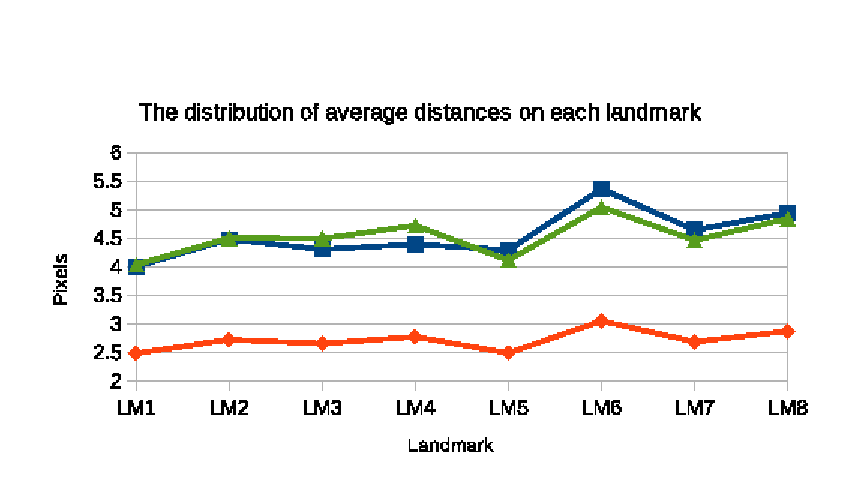
\includegraphics[scale=0.55]{images/prono_part}}
	\caption{The distribution of average distances on each landmark of pronotum part.}
	\label{figdistthorax}
\end{figure}

\begin{figure}[htbp]
	\centerline{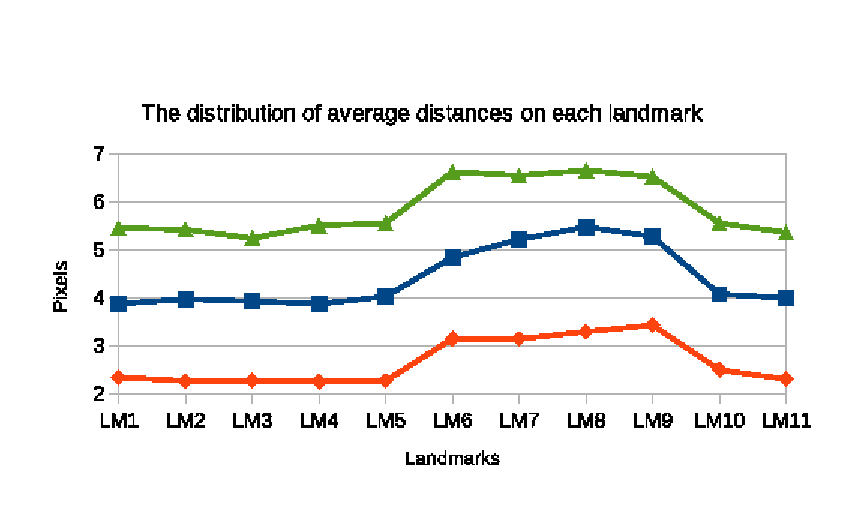
\includegraphics[scale=0.55]{images/body_part}}
	\caption{The distribution of average distances on each landmark of elytra part.}
	\label{figdistelytra}
\end{figure}

\begin{figure}[htbp]
	\centerline{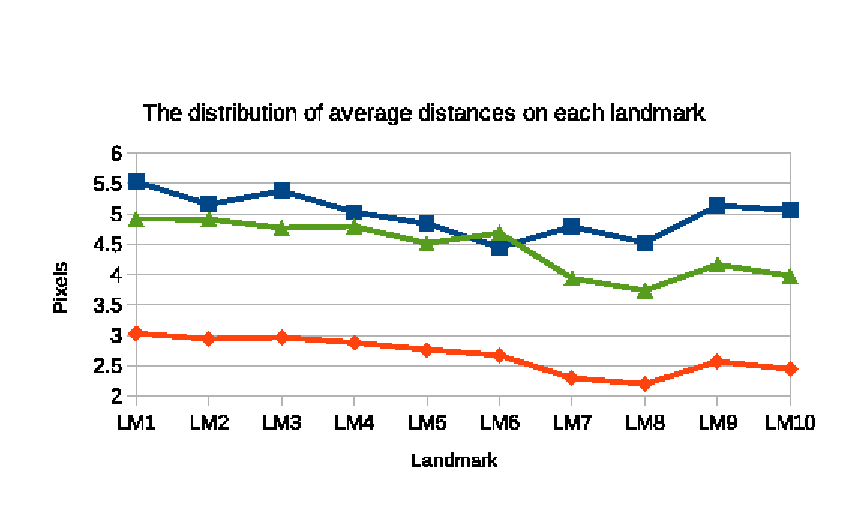
\includegraphics[scale=0.55]{images/head_part}}
	\caption{The distribution of average distances on each landmark of head part.}
	\label{figdisthead}
\end{figure}
\fi
\begin{figure}[htbp]
    \centering
    \subfloat[Left mandible]{\label{}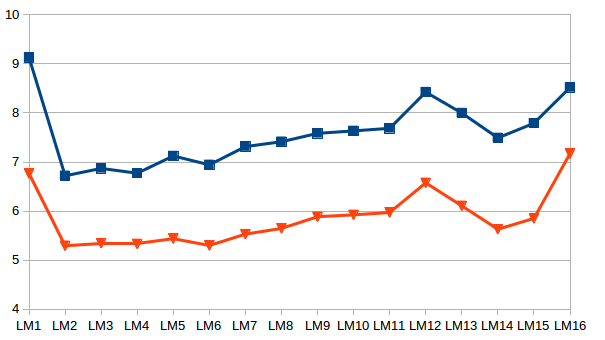
\includegraphics[width=0.5\textwidth]{images/mg_part}}~~
	\subfloat[Right mandible]{\label{}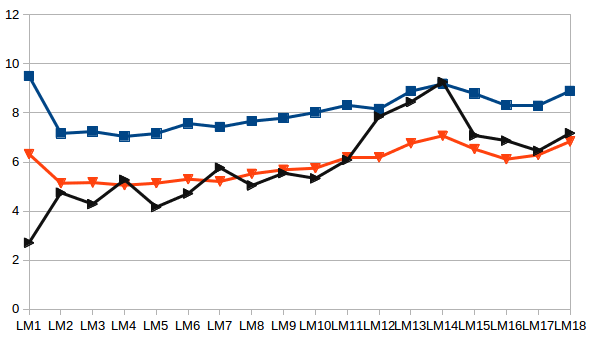
\includegraphics[width=0.5\textwidth]{images/md_part}}\\
    \subfloat[Head]{\label{}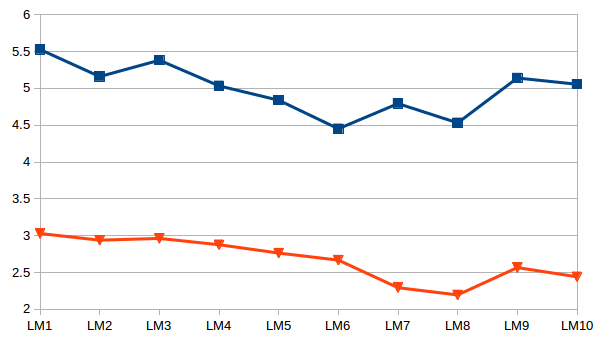
\includegraphics[width=0.5\textwidth]{images/tete_part}}~~
	\subfloat[Elytra]{\label{}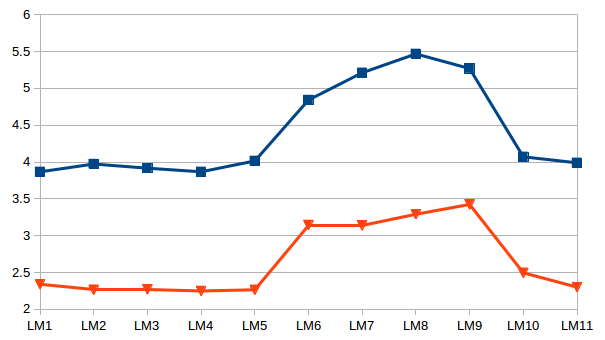
\includegraphics[width=0.5\textwidth]{images/elytre_part}}\\
	\subfloat[Pronotum]{\label{}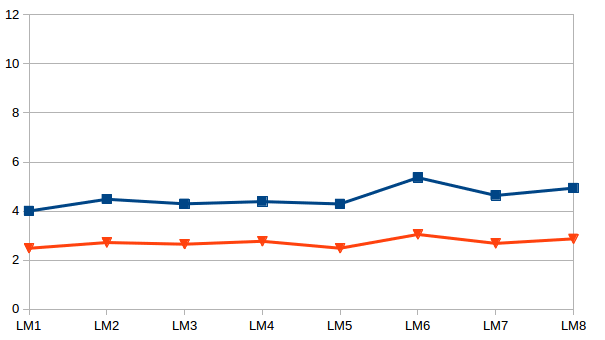
\includegraphics[width=0.5\textwidth]{images/pronotum_part.png}}
    \caption{The distribution of average distances on each landmark of each beetle's anatomical }
    \label{figdist5parts}
\end{figure}

The fine-tuning process has improved the results of the proposed architecture on both $5$ datasets: left, right mandible, pronotum, elytra and head. All the average distances are significantly decreased. Specially, the results have been improved $\approx 26.9\%$ on left mandible, $\approx 22.8\%$ on right mandible, $\approx 40.3\%$ on pronotum, $\approx 39.8\%$ on elytra, and $\approx 46.4\%$  on head part based on considering the average distances per landmark. Addition, in the cases of pronotum and head part, even if we plus the average distance and its standard deviation, the results are also less than the result when we trained the model from scratch. For segmentable images, we have a comparison between the results of deep learning and early method where we have applied image processing techniques to predict the landmarks. Clearly, the result with fine-tuning have improved the location of estimated landmarks, even when the average distances are still high when we trained the model from scratch: most of the average distance(or landmarks) of left mandibles are less than the results of the early method, while the average distances are very closed in the case of right mandibles.

To illustrate the final results, we display the distribution of
the distances in both cases: the best and the worst results (resp. landmark $1$ and $6$ on pronotum dataset) of five datasets (pronotum, elytra, head, left and right mandible) in  
%The Fig. \ref{figdist3parts} shows howmuch the average distances (blue lines) and standard errors (red lines) have been improved for the landmark 1 (Fig. (\ref{figdist3parts1}) and (\ref{figdist3parts2})) and landmark 6 (Fig. \ref{figdist3parts3}) and (\ref{figdist3parts4}).
Fig. \ref{figdist3parts}, \ref{figdist3partselytre}, \ref{figdist3partstete}, \ref{figdist3partsmg}, and \ref{figdist3partsmd}, respectively. In these figures, the left images present for the results when we trained the model from scratch; while the right images shows the results after applying fine-tuning. The blue lines in the charts present the average distance values. Clearly, the results in the fine-tuning case have been improved significantly than training from scratch.

\begin{figure}[htbp]
    \centering
    \subfloat[Landmark 1 - CNN]{\label{figdist3parts1}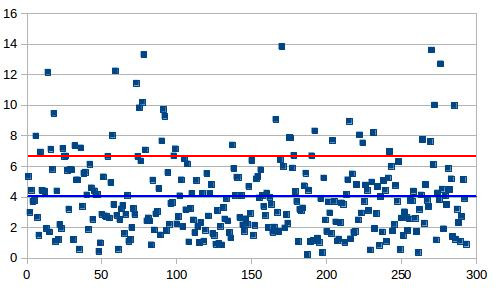
\includegraphics[width=0.5\textwidth]{images/lm1_cnn_2}}~~
	\subfloat[Landmark 1 - fine-tuning]{\label{figdist3parts2}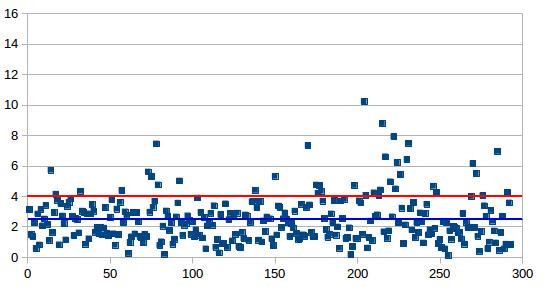
\includegraphics[width=0.5\textwidth]{images/lm1_finetuning_2}}\\
	\subfloat[Landmark 6 - CNN]{\label{figdist3parts3}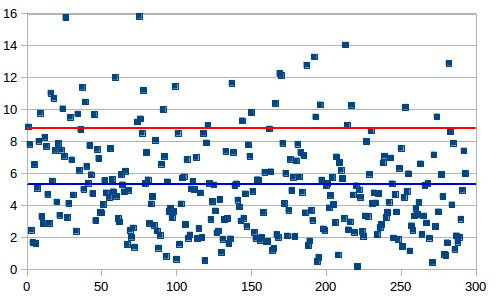
\includegraphics[width=0.5\textwidth]{images/lm6_cnn_2}}~~
	\subfloat[Landmark 6 - fine-tuning]{\label{figdist3parts4}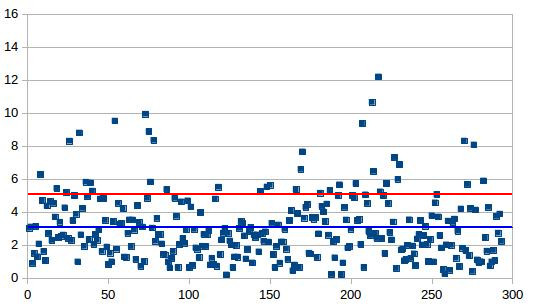
\includegraphics[width=0.5\textwidth]{images/lm6_finetuning_2}}\\
    \caption{The distribution of distances on $1^{st}$ and $6^{th}$
landmarks of all images in two testing steps (CNN and fine-tuning) (on \textbf{pronotum} dataset). The red line presents the standard deviation value.}
    \label{figdist3parts}
\end{figure}

\begin{figure}[htbp]
    \centering
    \subfloat[Landmark 1 - CNN]{\label{figdist3partselytre1}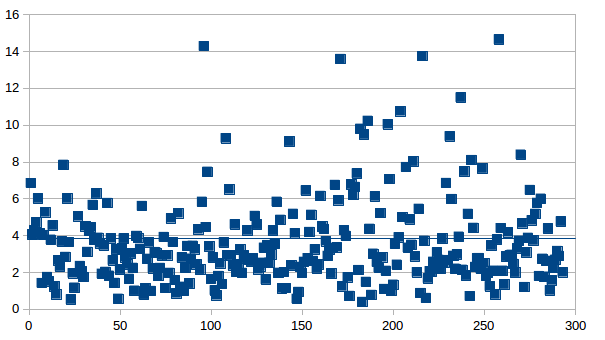
\includegraphics[width=0.4\textwidth]{images/fsc_elytre_lm1}}~~
	\subfloat[Landmark 1 - fine-tuning]{\label{figdist3partselytre2}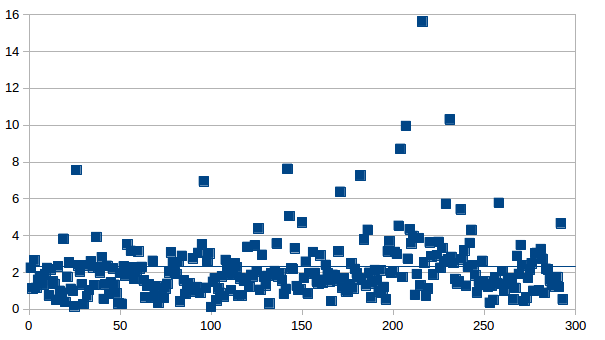
\includegraphics[width=0.4\textwidth]{images/fn_elytre_lm1}}\\
	\subfloat[Landmark 8 - CNN]{\label{figdist3partselytre3}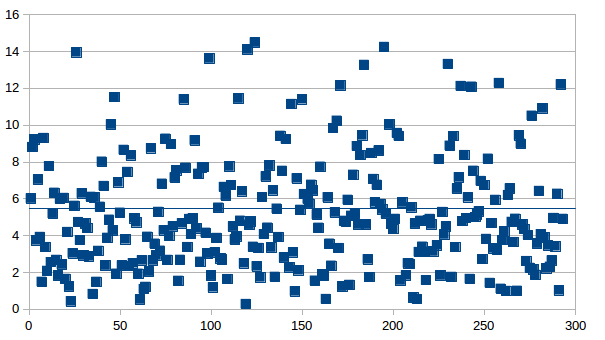
\includegraphics[width=0.4\textwidth]{images/fsc_elytre_lm8}}~~
	\subfloat[Landmark 8 - fine-tuning]{\label{figdist3partselytre4}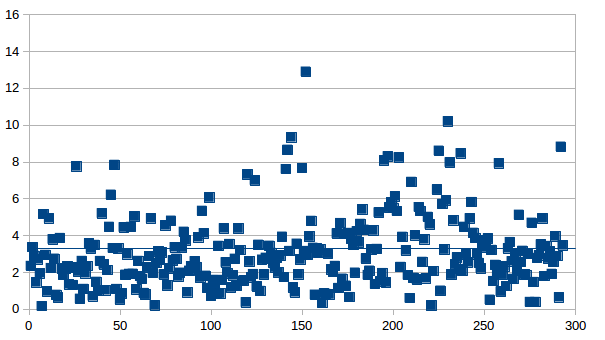
\includegraphics[width=0.4\textwidth]{images/fn_elytre_lm8}}\\
    \caption{The distribution of distances on $1^{st}$ and $8^{th}$
landmarks of all images in two testing steps (CNN and fine-tuning) (on \textbf{elytra} dataset).}
    \label{figdist3partselytre}
\end{figure}

\begin{figure}[htbp]
    \centering
    \subfloat[Landmark 1 - CNN]{\label{figdist3partstete1}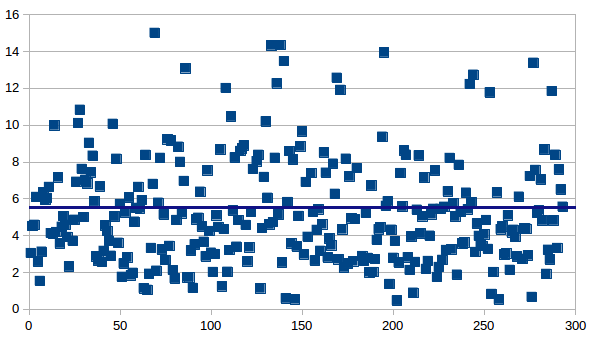
\includegraphics[width=0.4\textwidth]{images/fsc_tete_lm1}}~~
	\subfloat[Landmark 1 - fine-tuning]{\label{figdist3partstete2}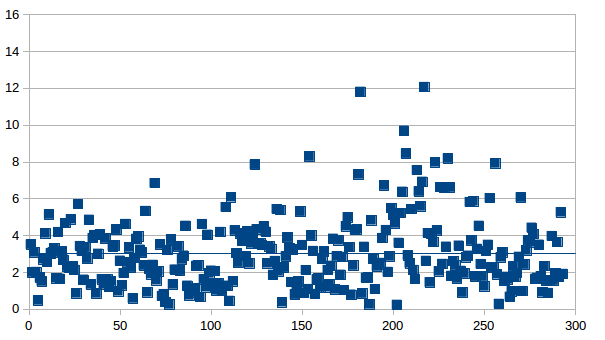
\includegraphics[width=0.4\textwidth]{images/fn_tete_lm1}}\\
	\subfloat[Landmark 6 - CNN]{\label{figdist3partstete3}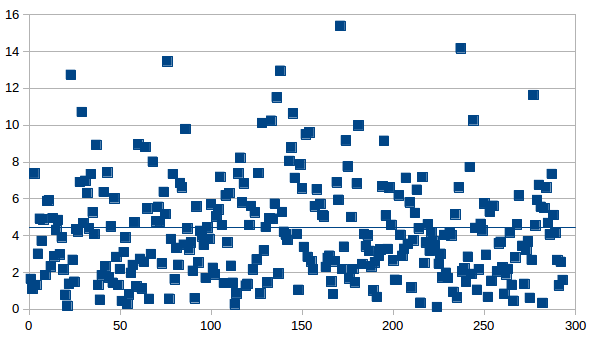
\includegraphics[width=0.4\textwidth]{images/fsc_tete_lm6}}~~
	\subfloat[Landmark 6 - fine-tuning]{\label{figdist3partstete4}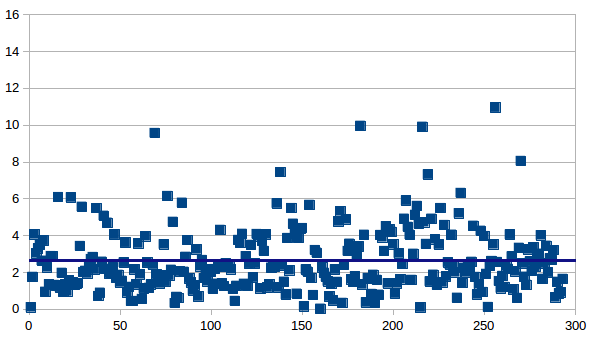
\includegraphics[width=0.4\textwidth]{images/fn_tete_lm6}}\\
    \caption{The distribution of distances on $1^{st}$ and $6^{th}$
landmarks of all images in two testing steps (CNN and fine-tuning) (on \textbf{head} dataset).}
    \label{figdist3partstete}
\end{figure}

\begin{figure}[htbp]
    \centering
    \subfloat[Landmark 4 - CNN]{\label{figdist3partstete1}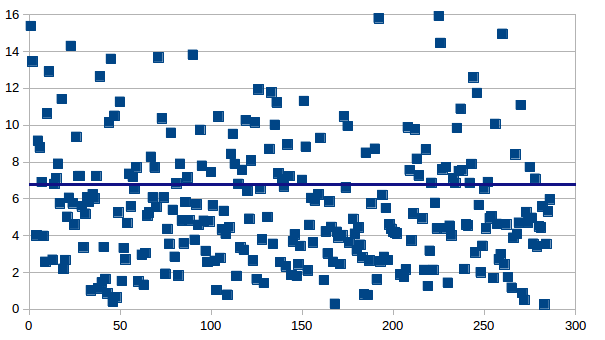
\includegraphics[width=0.4\textwidth]{images/fsc_mg_lm4}}~~
	\subfloat[Landmark 4 - fine-tuning]{\label{figdist3partstete2}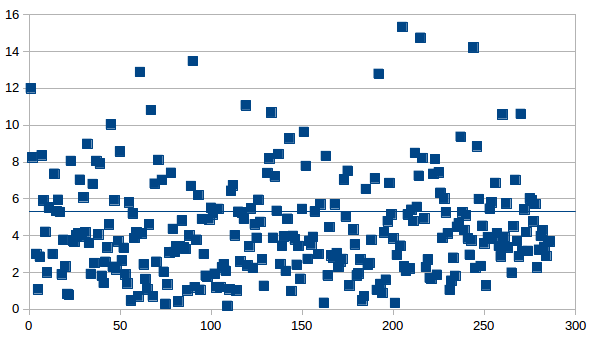
\includegraphics[width=0.4\textwidth]{images/fn_mg_lm4}}\\
	\subfloat[Landmark 1 - CNN]{\label{figdist3partstete3}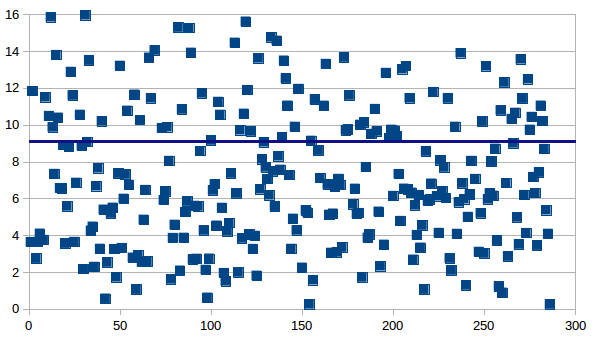
\includegraphics[width=0.4\textwidth]{images/fsc_mg_lm1}}~~
	\subfloat[Landmark 1 - fine-tuning]{\label{figdist3partstete4}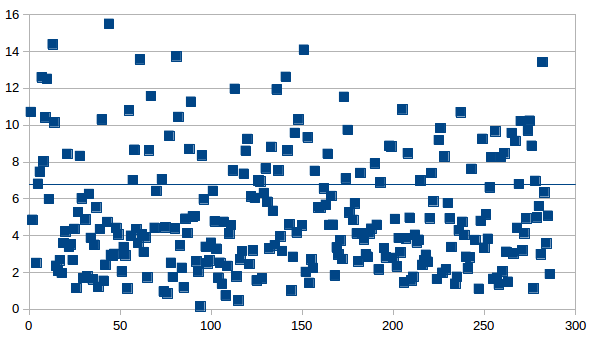
\includegraphics[width=0.4\textwidth]{images/fn_mg_lm1}}\\
    \caption{The distribution of distances on $1^{st}$ and $4^{th}$
landmarks of all images in two testing steps (CNN and fine-tuning) (on \textbf{left mandible} dataset).}
    \label{figdist3partsmg}
\end{figure}

\begin{figure}[htbp]
    \centering
    \subfloat[Landmark 4 - CNN]{\label{figdist3partstete1}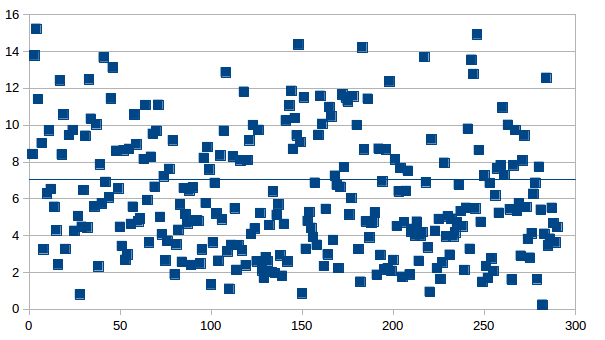
\includegraphics[width=0.4\textwidth]{images/fsc_md_lm4}}~~
	\subfloat[Landmark 4 - fine-tuning]{\label{figdist3partstete2}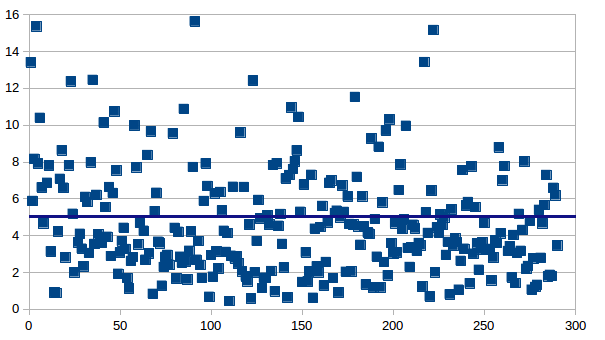
\includegraphics[width=0.4\textwidth]{images/fn_md_lm4}}\\
	\subfloat[Landmark 1 - CNN]{\label{figdist3partstete3}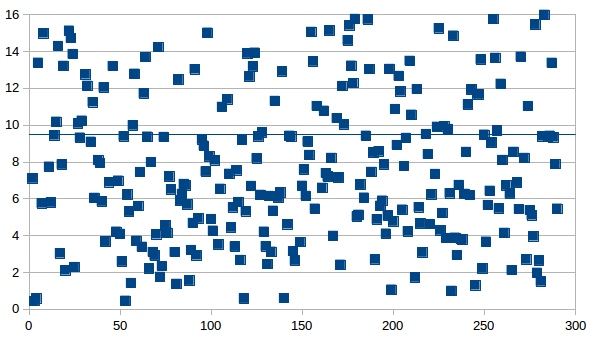
\includegraphics[width=0.4\textwidth]{images/fsc_md_lm1}}~~
	\subfloat[Landmark 1 - fine-tuning]{\label{figdist3partstete4}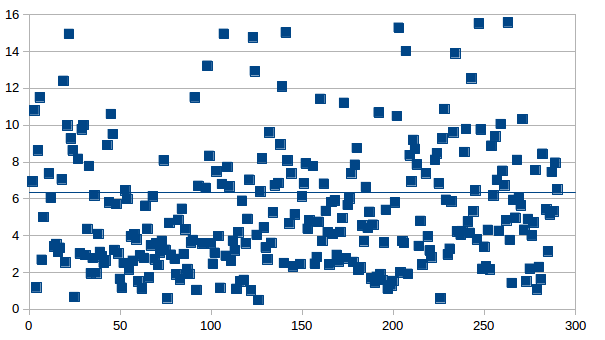
\includegraphics[width=0.4\textwidth]{images/fn_md_lm1}}\\
    \caption{The distribution of distances on $1^{st}$ and $4^{th}$
landmarks of all images in two testing steps (CNN and fine-tuning) (on \textbf{right mandible} dataset).}
    \label{figdist3partsmd}
\end{figure}

\pagebreak
\section{Conclusion}
\label{sconclusion}
In this work, we have presented how to apply convolutional neural network to predict the landmark on 2D anatomical images of beetles. After going through many trial models, we have presented a convolutional neural network for automatic detection landmarks on anatomical images of beetles which includes the repeated of some elementary blocks (an elementary block consists of a convolutional layer, a max pooling layer, and a dropout layer) followed by fully connected layers. Then, the proposed model have been trained and tested by using two strategies: \textit{train from scratch} and \textit{fine-tuning}. 

In our case, the size of dataset is limited. Therefore, we have applied the image processing techniques to augment dataset. The predicted landmarks have been evaluated by calculating the distance between manual landmarks and corresponding predicted landmarks. Then, the average of distance errors on each landmarks has been considered.

The results have been shown that using the convolutional network to predict the landmarks on biological images leads to satisfying results without need for segmentation step on the object of interest. The
best set of estimated landmarks has been obtained after a step
of fine-tuning using the whole set of images that we have for the
project, i.e. about all beetle parts. The quality of prediction allows using automatic landmarking to replace the manual ones.
\section*{References}

\bibliography{includes/mybibfile}

\end{document}




\begin{table}[htbp]
\begin{minipage}{0.5\linewidth}
	\centering
	\begin{tabular}{|c|c|}
		\hline
		\textbf{Landmark} & \textbf{Distance} (in pixels) \\ \hline
		1 & 3.8669  \\ \hline
		2 & 3.9730 \\ \hline
		3 & 3.9166 \\ \hline
		4 & 3.8673 \\ \hline
		5 & 4.0151 \\ \hline
		6 & 4.8426 \\ \hline
		7 & 5.2125 \\ \hline
		8 & 5.4685 \\ \hline
		9 & 5.2692 \\ \hline
		10 & 4.0709 \\ \hline
		11 & 3.9896 \\ \hline
	\end{tabular}
	\caption{\small{The average distance on all images per landmark on \textbf{elytra} images}}
	\label{tblavgdiselytra}
\end{minipage}
\hfill
\begin{minipage}{0.5\linewidth}
	\centering
	\begin{tabular}{|c|c|}
		\hline
		\textbf{Landmark} & \textbf{Distance} (in pixels) \\ \hline
		1 & 5.5280  \\ \hline
		2 & 5.1609 \\ \hline
		3 & 5.3827 \\ \hline
		4 & 5.0345 \\ \hline
		5 & 4.8393 \\ \hline
		6 & 4.4516 \\ \hline
		7 & 4.7937 \\ \hline
		8 & 4.5322 \\ \hline
		9 & 5.1412 \\ \hline
		10 & 5.0564 \\ \hline
	\end{tabular}
	\caption{\small{The average distance on all images per landmark on \textbf{head} images}}
	\label{tblavgdishead}
\end{minipage}
\end{table}

\begin{table}[htbp]
\begin{minipage}{0.5\linewidth}
	\centering
	\begin{tabular}{|c|c|}
		\hline
		\textbf{Landmark} & \textbf{Distance} (in pixels) \\ \hline
		1 & 9.1267  \\ \hline
		2 & 6.7198 \\ \hline
		3 & 6.8704 \\ \hline
		4 & 6.7719 \\ \hline
		5 & 7.1250 \\ \hline
		6 & 6.9441 \\ \hline
		7 & 7.3158 \\ \hline
		8 & 7.4142 \\ \hline
		9 & 7.5846 \\ \hline
		10 & 7.6349 \\ \hline
		11 & 7.6873 \\ \hline
		12 & 8.4248 \\ \hline
		13 & 7.9983 \\ \hline
		14 & 7.4919 \\ \hline
		15 & 7.7903 \\ \hline
		16 & 8.5198 \\ \hline
	\end{tabular}
	\caption{\small{The average distance on all images per landmark on \textbf{left mandible} images}}
	\label{tblavgdislmandible}
\end{minipage}
\hfill
\begin{minipage}{0.5\linewidth}
	\centering
	\begin{tabular}{|c|c|}
		\hline
		\textbf{Landmark} & \textbf{Distance} (in pixels) \\ \hline
		1 & 9.4981  \\ \hline
		2 & 7.1657 \\ \hline
		3 & 7.2420 \\ \hline
		4 & 7.0436 \\ \hline
		5 & 7.1599 \\ \hline
		6 & 7.5699 \\ \hline
		7 & 7.4251 \\ \hline
		8 & 7.6636 \\ \hline
		9 & 7.7906 \\ \hline
		10 & 8.0197 \\ \hline
		11 & 8.3140 \\ \hline
		12 & 8.1564 \\ \hline
		13 & 8.8879 \\ \hline
		14 & 9.1842 \\ \hline
		15 & 8.7875 \\ \hline
		16 & 8.3141 \\ \hline
		17 & 8.2866 \\ \hline
		18 & 8.8928 \\ \hline
	\end{tabular}
	\caption{\small{The average distance on all images per landmark on \textbf{right mandible} images}}
	\label{tblavgdisrmandible}
\end{minipage}
\end{table}